\documentclass[main.tex]{subfiles} \newcommand{\D}{\mathcal{D}}
\newcommand{\Kc}{\mathcal{K}} \newcommand{\Lc}{\mathcal{L}} \begin{document}

\section{Stabilité de Lagrange} Le premier a avoir introduit la notion de
stabilité est Lagrange.  Le concept est basé sur l'énergie potentielle $V$.
Puisque les points d'équilibre du système correspondent aux points tels que
$\derivp[V]{q}=0$ avec $q$ les coordonnées généralisées du mouvement, alors un
point d'équilibre est stable suivant Lagrange si $\derivpp[V]{q} > 0$

\begin{figure}[H] \centering 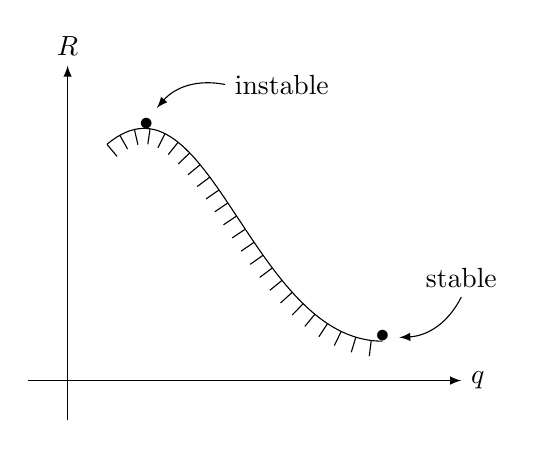
\begin{tikzpicture} \draw[-latex] (-0.5,0) --
	(5,0) node[right]{$q$}; \draw[-latex] (0,-0.5) -- (0,4) node[above]{$R$};
	\draw (0.5,3) to[out=40,in=180] (4,0.5); \draw[decorate,
	decoration={border,amplitude=-0.2cm,angle=90,segment length=0.2cm}] (0.5,3)
	to[out=40,in=180] (4,0.5); \node(I) at (1,3.26) {$\bullet$}; \node(S) at
(4,0.56) {$\bullet$}; \draw[latex-] (I) to[bend left] ++ (1,0.5)
node[right]{instable}; \draw[latex-] (S) to[bend right] ++ (1,0.5)
node[above]{stable}; \end{tikzpicture} \caption{Stabilité au sens de Lagrange}
\end{figure}

Suivant Lagrange, un point d'équilibre est stable si pour toutes conditions
initiales, la trajectoire reste bornée.

\begin{itemize} \item On contrôle la variation sur la trajectoire par celle sur
la condition initiale.  \item des petites variation sur la condition initiale
implique de petite variation sur la trajectoire.  \end{itemize}

\begin{rem} La notion de stabilité en non linéaire concerne les points
d'équilibre et non le système. Mathématiquement, Dirichlet a formalisé la
stabilité au sens de Lagrange avec les trajectoires.  \end{rem} \newpage
\begin{defin} Un point d'équilibre $x^*$ est stable au sens de Lagrange si et
	seulement si

  \[\forall \delta > 0, \exists \varepsilon > 0 \text{ tel que } \forall t \in
\R, || x_0-x^* || \leq \delta \Rightarrow ||\chi(t,\chi(t_0,x_0))-x^* || \leq
\varepsilon\] \end{defin}

Ainsi la stabilité suivant Lagrange est qu'un petit changement borné sur $x^*$
implique un petit changement borné sur la trajectoire.

\[\forall \delta > 0, \exists \epsilon > 0 \text{ tel que }  ||\chi(t_0,x_0)||
\leq \delta \Rightarrow ||\chi(t,\chi(t_0,x_0))|| \leq \epsilon \]

Sans perte de généralité, on considère le point d'équilibre $x^* = 0$.


\begin{rem} La stabilité suivant Lagrange n'implique pas la convergence mais
seulement la bornitude\footnote{sic.} (la trajectoire reste bornée), ce n'est
pas suffisant pour faire de l'automatique, il faut pouvoir garantir la
convergence. On utilise donc la stabilité au sens de Lyapounov \end{rem}

\section{Stabilité au sens de Lyapunov}

\begin{defin} \[\forall \epsilon > 0, \exists \delta > 0 \text{ tel que }
||\chi(t_0,x_0)|| \leq \delta \Rightarrow || \chi(t,\chi(t_0,x_0)) || \leq
\epsilon\] \end{defin}

Attention : il n'y a pas d'implication entre les deux.

\begin{rem} C'est $\varepsilon$ qui contrôle $\delta$.  \end{rem} \begin{rem}
	La condition de Lagrange est sur la bornitude de la trajectoire (quelles
	que soient les conditions initiales, on borne la solution). Par contre, la
	condition de Lyapunov est sur la convergence dans un voisinage (il existe
	des conditions initiales pour lesquelles les trajectoires convergent vers
	$x^*$).  \end{rem}

\begin{exemple}[Oscillateur de Van der Pol] \[ \begin{cases} \dot{x_1} & =
x_2\\ \dot{x_2} & = -x_1 + (1-x_ 1^2)x_2 \end{cases} \]

  Point d'équilibre $x^* =(0,0)$

  \begin{rem} Il n'existe pas de solution analytique aux équations de Van der
  Pol, mais numériquement on trouve un cycle limite stable.  \end{rem}

  % \img{0.3}{3/2.png}

  $\exists \epsilon$ tel que le cycle limite $\subset$ cercle de centre (0,0)
  et de rayon $\epsilon$ : stable au sens de Lagrange. Par contre, pas stable
  au sens de Lyapunov car on a \[ \forall \delta > 0, \nexists \epsilon > 0
  \text{ tel que } ||\chi(t,\chi(t_0,x_0))|| < \epsilon \]

\end{exemple}

\begin{exemple}[Pendule sans frottement] L'origine est stable suivant Lyapunov
	avec $\delta = \epsilon$.

  Elle n'est pas stable suivant Lagrange \[x_0=(x_1= \pi, x_2=0) : \nexists
\epsilon >0 \text{ tel que } \|\chi(t,\chi(0,s_0))\| < \epsilon \]
\end{exemple}

\subsection{Stabilité uniforme} \begin{defin} Le point d'équilibre $x^* (x^*
	=0)$ est dit point d'équilibre uniformément stable si, pour la condition de
	Lyapunov, $\delta$ peut être choisi indépendamment des conditions initiales
	$t_0,x_0$ \end{defin}


\begin{defin} On définit les \emph{fonctions de caractérisations} suivantes :
\begin{enumerate} \item Si $\alpha : \R_+ \rightarrow \R_+$ est continue et
			strictement croissante, $\alpha$ est dite de classe $\Kc$.

	Si $\alpha$ croit indéfiniment (i.e. $\alpha (s) \rightarrow \infty$),
		alors $\alpha\in \Kc_{\infty}$

  \item $\phi$ est dite de classe $\Lc$ si $\phi:\R_+\rightarrow\R_+$ continue,
	  strictement décroissante et $\phi(s) \rightarrow 0$

  \item $\beta$ est dite de classe $\Kc\Lc$ si $\beta:\R_+ \times \R_+
	  \rightarrow \R_+$ si $\beta(.,r)\in \Lc \text{ et } \beta(s,.) \in \Kc$

	Typiquement $\beta(s,r)=\alpha(s).\phi(r) \text{ avec } \alpha\in\Kc, \phi
\in \Lc$.  \end{enumerate} \end{defin}

\begin{exemple} $\beta(\|x_0\|,|t|)=\|x_0\|e^{-\lambda |t|} \text{ avec }
	\lambda >0$

  Ainsi le but est d'arriver à vérifier pour une trajectoire du système $
\|\chi(t,x_0)\| \leq \beta(\|x_0\|,t),t \geq 0$ (enveloppe) \end{exemple}

\begin{prop} L'origine est uniformément stable si et seulement si \[\exists
c>0, \alpha \in \Kc \text{ tel que } \|\chi(t_0,x_0)\| \leq c \Rightarrow
\|\chi(t,\chi(t_0,x_0))\| \leq \alpha (\|\chi(t_0,x_0)\|)\] \end{prop}

\begin{proof} Condition suffisante.

  Soit $\alpha \in \Kc$ (strictement croissante et continue, donc $\alpha^{-1}$
	existe).

  Pour $\epsilon >0, \exists \delta$ dépendant de $\epsilon \text{ tel que }
	\delta = \alpha^{-1}(\epsilon)$.

  Si $\|\chi(t_0,x_0)\| \leq \delta \Rightarrow \|\chi(t,\chi(t_0,x_0))\| \leq
	\alpha(\alpha^{-1}(\epsilon)) \leq \epsilon$\\

  Condition nécessaire.

  $\forall \epsilon>0, \exists \delta$ dépendant de $\epsilon \text{ tel que }
	\|s_0\| \leq \delta \Rightarrow \|s\| \leq \epsilon$

  Si $\epsilon_2 > \epsilon_1 \Rightarrow \delta_2 \geq \delta_1$ (suivant
	Lyapunov). On définit $\delta' \in \Kc \text{ tel que } \delta'<\delta$.

  Pour $\epsilon > 9, \exists \delta > 0 \text{ tel que }$ \begin{align*}
  \|s_0\| \leq \delta & \Rightarrow \|\delta\| \leq \epsilon\\ \|s_0\| \leq
  \delta' & \Rightarrow \|\delta\| \leq \epsilon \text{ car } \delta'<\delta
  \end{align*}

  Si on définit $\alpha(\|.\|)=(\delta')^{-1}$, $\forall \epsilon >0, \exists
	\delta'(\epsilon)$ où $\|s_0\|=\delta'(\epsilon) \Rightarrow \epsilon =
	(\delta')^{-1}(\|s_0\|)$

  Suivant Lyapunov, cela implique $\|s\| \leq \epsilon \leq \alpha (\|s_0\|)$
\end{proof}

\section{Attractivité (convergence)} \begin{defin} $\exists r > 0, \forall
	\sigma > 0, \exists T > 0 \text{ tel que } \|\chi(t_0,x_0)\| \leq r
	\Rightarrow \|\chi(t,\chi(t_0,x_0))\| \leq \sigma, \forall t \geq T$

  % \img{0.5}{4/1.png}

  Autrement dit : $\|s_0\| \leq r \Rightarrow \lim_{t\rightarrow \infty}
	\|\chi_t\| = 0$.

  On parle d'attractivité uniforme si $T$ ne dépend pas de $t_0$.  \end{defin}

\begin{prop}[Stabilité asymptotique] L'origine est asymptotiquement stable si
et seulement si \begin{itemize} \item stabilité au sens de Lyapunov et
		attractivité \item $\|s_0\| \leq r \Rightarrow \|s\| \leq \beta
			(\|s_0\|,t), \quad \beta \in \Kc\Lc$ \end{itemize} \end{prop}

\begin{prop}[Stabilité exponentielle] L'origine est exponentiellement stable si
et seulement si \begin{itemize} \item stabilité au sens de Lyapunov et
		attractivité \item $\exists \alpha, \lambda, r >0 \text{ tel que }
			\|s_0\| \leq r \Rightarrow \|s\| \leq \alpha \|s_0\| e^{-\lambda
			t}$ \end{itemize} \end{prop} \begin{prop}[Stabilité locale et
				globale] \begin{itemize} \item L'origine est globalement stable
							si la stabilité (asymptotique, exponentielle,...)
							ne dépend pas de la condition initiale, i.e.
							$\forall t_0 \in \R \text{ et } x_0 \in \R^n$ et
							dit localement stable (asymptotiquement,
							exponentiellement,...) \item Si la stabilité dépend
				de la CI, i.e. $\exists V_t \subset \R$ ou $V_x \in \R^n$ tel
				que $\forall t_0 \in V_t$ et $\forall x_0 \in V_x$, l'origine
				est stable.  \end{itemize} \end{prop} \paragraph{Problème}
				Généralement, on n'a pas de solution analytique de l'équation
				différentielle. Ainsi, la stabilité ne peut pas être vérifiée
				via la trajectoire.

\begin{defin} $V$ est une \emph{fonction de Lyapunov} si : \begin{enumerate}
	\item $V : \begin{cases} \R^n & \rightarrow \R_+\\x & \mapsto V(x)
	\end{cases} $ telle que $V(0)=0$ et $V(x) \geq 0$ (définie semi-positive)
		ou telle que $V(0)=0$ et $V(x) > 0$ si $x\neq 0$ (définie positive)
\item $V$ est radialement non bornée, i.e. $V(x) \rightarrow_{\|x\| \rightarrow
\infty} \infty$ \end{enumerate} \end{defin}

\begin{thm}[Stabilité au sens de Lyapunov] Soit $\dot{x}(t) = f(x(t))$ et
	$f(0)=0$ (origine est un point d'équilibre). On suppose qu'il existe $V$
	(fonction de Lyapunov) continue et différentiable tel que \[ \exists D
	\subset \R^n, 0 \in \D \text{ où } \forall x \in \D, \quad \dot{V}(x) =
	(\derivp[V]{x})^Tf(x) \leq 0 \] Alors l'origine est stable au sens de
	Lyapunov sur $\D$.

  Si $\D = \R^n$, 0 est globalement stable au sens de Lyapunov.  \end{thm}

\begin{proof} Si $x=0$ est stable, alors $\forall \epsilon > 0, \exists \delta
	> 0 \text{ tel que } \|s_0\| \leq \delta \Rightarrow \|s\| \leq \epsilon$.

  Pour $\epsilon > 0$ on définit $0<r\leq \epsilon$ avec $B_r(0) = \{ x \in \D
	\text{ tel que } \|x\| \leq r \}$

  Soit $\alpha = \min_{\|x\| = r} V(x)$ et on choisit $\beta$ tel que $\beta <
	\alpha$ et on définit $\Omega_{\beta} = \{ x \in B_r(0) \text{ tel que }
	V(x) \leq \beta \}$.

  $0\in \Omega_{\beta}$ car $V(0) = 0$ et $\Omega_{\beta} \subset B_r(0)$.

  Soit $x_0\in \Omega_{\beta} \subset \D$ : $\dot{V}(x) \leq 0$ \begin{align*}
	  \Rightarrow & V(x(t)-V(x_0) \leq 0 \quad (\text{ car } \in \D) \\
	  \Rightarrow & V(x(t)) \leq V(x_0) \leq \beta \quad (\text{ car } x_0 \in
	  \Omega_{\beta}) \\ \Rightarrow & x(t) \in \Omega_{\beta} \subset B_r(0)\\
  \Rightarrow & \|x(t)\| \leq \epsilon \quad r \leq \epsilon \end{align*}

  (Autrement dit si on part de $\Omega_{\beta}$ on reste dans $\Omega_{\beta}$)

  $\delta(\epsilon)$ est le rayon de la boule de centre O et $\subset
\Omega_{\beta}$ \end{proof}

\begin{thm}[Stabilité asymptotique au sens de Lyapounov] Soient le système
	$G:\dot{x}=f(x)$ et $f(0)=0$ et $V:\D \rightarrow\R_+$ une fonction de
	Lyapunov continue et différentiable telle que \[ \forall x \in \D, \quad
	\dot{V}(x) = (\derivp[V]{x})^T f(x) \leq -Q(x), \quad \text{ où } Q(x)
	\text{ est définie positive } \]

  Alors l'origine est asymptotiquement stable.  \end{thm}


\begin{rem} $Q(x)$ dépend de toutes les variables d'état. Sinon la convergence
asymptotique n'est vérifié que pour certaine direction.  \end{rem}


\begin{exemple}[Cas linéaire]

  $\dot{x}=Ax$ avec $x\in \R^n$

  Soit $P$ une matrice semi définie positive ($P^T = P \text{ et } \lambda(P) =
	0 \Leftrightarrow \forall x\in \R^n, x^T P x \geq 0$)

  On définit $V(x) = x^TPx$ fonction de Lyapunov

  \begin{align*} \dot{V}(x) & = \dot{x}^T P x + x^T P \dot{x} \\ & = x^T APx +
  x^T PAx \\&= x^T(A^TP + PA)x \end{align*}

  \emph{Suivant Lyapunov, A est Hurwitz si et seulement si $Re(\lambda(A)) <
	0$}.

  $\exists P > 0 \text{ tel que } A^TP + PA$ définie négative.

  On pose $P = \int_0^{\infty} e^{A^Tt}Qe^{At} dt$ avec $Q$ définie positive.
	On a donc $P$ définie positive.

  \[ \int_0^{\infty} (A^T e^{A^Tt} Q e^{At} + e^{A^T t} Q e^{At} A)dt =
	\int_0^{\infty} \dd{e^{A^Tt} Q e^{At}}{t} dt =
	\left[e^{A^Tt}Qe^{At}\right]_0^{\infty}\]

  Si $A$ est Hurwitz : $e^{At} \xrightarrow[t\rightarrow \infty]{} 0$

  \[A^T P + PA = -Q \text{ définie négative (équation de Lyapunov)} \]

  Pour le système linéaire \[ \dot{V}(x) = x^T (A^T P + PA)x \leq -x^T Q x\]
	$\Rightarrow$ Stabilité de Lyapunov $\Leftrightarrow$ Stabilité
	asymptotique

\end{exemple}

\begin{thm}[Stabilité exponentielle] Soient le système $G: \dot{x}=f(x)$ et
$f(0)=0$, $\exists V : \D \rightarrow \R_+$ fonction de Lyapunov continue et
différentiable telle que \begin{enumerate} \item $\exists \alpha > 0, \beta >
			0$ et $c\geq 1$ tel que \[ \quad \forall x \in \D, \quad \alpha
\|x\|^c \leq V(x) \leq \beta \|x\|^c\] \item $\exists \gamma > 0$ tel que \[
\quad \forall x \in \D, \dot{V} \leq - \gamma V \leq - \gamma \|x\|^c \]
\end{enumerate} Alors l'origine est exponentiellement stable. Si $\D=\R^n$, on
	a aussi la stabilité globale.  \end{thm}

\begin{proof} $\dot{V} \leq -\gamma V \Rightarrow V(x(t)) \leq
	V(x(0))e^{-\gamma t}$

  si $\dot{\hat{V}}=-\gamma \hat{V}$ \begin{align*} V(x(0)) & \leq \beta
	  \|x(0)\|^c \\ \text{ et } V(x(t)) & \geq \alpha \|x(t)\|^c \\
	  V(x(0))e^{-\gamma t} & \geq \\ \beta\|x(0)\|^c e^{-\gamma t} & \geq
	  \qquad \Rightarrow \|x(t)\| \leq
	  (\frac{\beta}{\alpha})^{1/c}\|x(0)\|e^{-\frac{\gamma}{c}t} \end{align*}
\end{proof}

\begin{corol} Le syst linéaire est aussi exponentiellement stable: \[ V = x^T P
x \implies \alpha \|x\| \le V(x) \le \beta \|x\|^c \] Avec $\alpha$ plus petite
valeur propre de $P$ et $\beta$ plus grande valeur propre de $P$.  \end{corol}
si on a la stabilité asymptotique \[ \dot{V}=x^T(A^TP+PA)x x^T R x \le -\gamma
V x^T R x \le -\gamma \|x\|^2 \] \begin{exemple} $\begin{cases} \dot{x_1} & =
	-x_1^3 + x_2 ^3 + x_1x_2^2\\\dot{x_2} & = - x_2^2 x_1 - 5x_2^3 \end{cases}$


  $(x_1,x_2)=(0,0),f(0)=0$ est-il asymptotiquement stable ?

  On pose $V(x) = \frac{1}{2}(x_1^2 + x_2^2)$. $V(0) = 0$ et $V(x)>0, \forall x
  \neq 0$.

  \[ \dot{V}(x) = x_1\dot{x_1} + x_2 \dot{x_2} = -x_1^4 + x_1^2 x_2^2 - 5 x_2^4
  \leq -\frac{1}{2}x_1^4 - \frac{9}{2}x_2^4 \leq - Q(x) \text{ tel que } Q(x)
  \geq 0 \]

  L'origine est globalement asymptotiquement stable.\\

  Est-il exponentiellement stable ?

  \[ \alpha \|x(t)\|^c \leq V(x(t)) \leq \beta \|x(t)\|^c \]

  $\beta=1,\alpha=\frac{1}{4}$

  \[ \dot{V} \leq - \frac{1}{2}x_1^4 - \frac{9}{2}x_2^4 \leq -\frac{9}{2}(x_1^4
  + x_2^4) \]

  Pour $\D = \{ \|x\| \leq 1 \}, x_1^2 +x_2^2 \geq x_1^4 + x_2^4$ donc $-(x_1^2
  + x_2^2) \leq -(x_1^4+x_2^4)$ : on ne peut pas borner $\dot{V}$ par $V$.

  Avec ce $V(x)$ on ne peut décider de la convergence exponentielle.
  \end{exemple}

Si on arrive pas a vérifier la stabilité alors le point d'équilibre (ou
l'origine) peut-être instable. Dans ce cas, comment vérifier l'instabilité du
point d'équilibre (origine)?\\

\begin{thm}[Théorème de Lyapunov d'instabilité] Soit le système G: $x=f(x)$,
	$f(0)=0$ et $t\geq 0$.  Si $\exists V : \D \subset \mathbb{R}^n \rightarrow
	\mathbb{R}_+$ continue, différentiable et définie positive ($0 \in \D$),
	tel que \[\forall x \in \D^*, \quad  \dot{V}(x) = \left( \frac{\partial
V}{\partial x}\right)^T f(x) >0 \] alors l'origine est instable.  \end{thm} Le
système accumule de l'énergie et deviens instable \begin{proof} Instable
	$\Leftrightarrow$ $\exists \epsilon>0$ tel que $\forall \delta >0$, alors
	$\|x_0\| \leq \delta$ et $\|x\| \geq \epsilon$\\

  $\forall \delta > 0$ soit $r \in ]0;\delta[$ tel que:\\ $B_r(0) = \{ x\in \D$
	tel que $ \|x\| \leq r \}$ est compact.\\ On pose $\alpha = max_{B_r(0)}
	V(x)$ et $x_0 \in B_r(0)$\\ $V(x_0) = \alpha$, ainsi $V(x) - V(x_0) >0$ :
	\begin{align*} \Rightarrow & V(x) > \alpha\\ \Rightarrow & x \notin B_r(0)
	\\ \Rightarrow & x \in B_r^c(0)\\ \Rightarrow & \|x\|> r \end{align*} Donc
$\exists \epsilon >0$ tel que $\|x\| \geq \epsilon > r$ \end{proof}
\subsection{Théorème simplifiant l'analyse de la stabilité}


\begin{thm}[Théorème de Barbashin-Krasovsky (Stabilité asymptotique)] Soit
	$\{0\}$ un point d'équilibre du système $\dot{x} = f(x)$ , où $f:\D
	\rightarrow \mathbb{R}^n$, localement lipschitzienne. On suppose qu'il
	existe $V$ continue, différentiable et définie positive telle que \[\dot{V}
	\leq 0\] Soit $S = \{x \in \D$ tel que $\dot{V(x)} = 0\}$.

  Si $x=0$ est le seul élément de $S$, alors l'origine est asymptotiquement
stable.  \end{thm}

\begin{exemple} Soit le système : \[ \begin{cases} \dot{x_1} &= -x_1^3 + 2
x_2^3\\\dot{x_2} &= -2x_1x_2^2 \end{cases} \] L'origine est un point
d'équilibre.\\ \begin{align*} V(x) &= \frac{1}{2}x_1^2 + \frac{1}{2}x_2^2 >0\\
	\dot{V(x)} &= x_1\dot{x_1} + x_2\dot{x_2} = -x_1^4 \leq 0 \end{align*} On
	ne peut pas conclure sur la stabilité asymptotique car $Q(x) =
	\frac{1}{2}x_1^4$ ne dépend pas de $x_2$. \\

  On utilise le théorème de Barbashin : \begin{align*} S = \{x \in \D \text{
		  tel que }\dot{V(x)} = 0\} \Rightarrow x_1 = 0\\ \Rightarrow &
	  \dot{x_2} = 0\\ \Rightarrow & x_2 = 0\\ \Rightarrow & S = \{0\}\\
	  \Rightarrow & \text{Stabilité asymptotique} \end{align*} \end{exemple}

\begin{thm}[Principe d'invariance de LaSalle] Soient $ \dot{x} = f(x)$ avec $f:
	\D \rightarrow \mathbb{R}^n$, $\Omega$ un compact positivement invariant
	tel que $\Omega \subset \D$, $V:\D\rightarrow\mathbb{R}_+$ continue,
	différentiable tel que $\dot{V} \leq 0 $ dans $\Omega$, $E= \{x \in \Omega$
	tel que $ \dot{V}=0\}$ et M le plus grand ensemble positivement invariant
	inclus dans E.

  Alors toute solution $x$ tel que $x_0 \in \Omega$ converge vers M quand $t
\longrightarrow \infty$. Autrement dit $\overline{M}$ est l'attracteur.
\end{thm}


\begin{exemple}[Barbashin] Soit le système \[ \begin{cases} \dot{x_1} & =x_2\\
\dot{x_2} & = -h(x_1) - g(x_2) \end{cases} \] où $h,g:[-a,a] \rightarrow \R$
avec $h(0)=g(0)=0$

  et $\forall x \neq 0, \quad x.h(x) >0 \text{ et }  x.g(x) >0$.\\

  L'origine est un point d'équilibre.\\

  Fonction de Lyapunov candidate : \[ V(x) = \int_0^{x_1} h(s)ds +
  \frac{1}{2}x_2^2 \]

  $x_1 = 0$ et $x_2=0 \Rightarrow V(x)=0$

  $x_1 \neq 0$ ou $x_2 \neq 0 \Rightarrow V(x) > 0$

  donc $V$ est définie positive.\\

  \begin{align*} \dot{V}(x) & = h(x_1) \dot{x_1}+ x_2 \dot{x_2}\\ & = h(x_1)x_1
  - x_2h(x_1) - g(x_1)x_2 \\ & = -g(x_2)x_2 \leq -Q(x) \text{ définie positive,
  dépend de } x_1 \text{ et } x_2 \end{align*}

  Barbashin :

  $E = \{ x \in  \R^2, \dot{V}(x) = 0 \}$

  $\dot{V}(x)=0 \Rightarrow x_2 = 0 \Rightarrow \dot{x_1}=0$

  $\dot{x_2} = 0 + x_2 = 0 \Rightarrow h(x_1)=0 \Rightarrow x_1 = 0$

  Alors $E=\{0\}$ stabilité asymptotique globale.  \end{exemple}

\begin{exemple}[Invariance de La Salle] Soit le système $\dot{x} = ax + u$, $a$
	inconnu mais borné.

  $u=-kx$ et $\dot{k}= \gamma x^2, \gamma >0$

  On pose $x_1=x$ et $x_2=k$ \[ \begin{cases} \dot{x_1} & = ax_1 - x_2x_1
  \\\dot{x_2}&  = \gamma x_1^2 \end{cases} \]

  La fonction de Lyapunov candidate \[ V(x) = \frac{1}{2} x_1^2 +
	\frac{1}{2\gamma} (x_2-b)^2, \quad \text{ avec } b>a \text{ car $a$ est
	borné} \] $V(0,b)=0$ et non pas l'origine

  $V(x) \geq 0, \forall x \in \R^d$ \begin{align*} \dot{V}(x) & = x_1 \dot{x_1}
  + \frac{1}{\gamma}(x_2-b)\dot{x_2} \\ & = ax_1^2 - x_1^2 x_2 + (x_2-b)x_1^2
  \\ & = x_1^2 (a-b) \leq 0 \end{align*}

  $E = \{ x \in \R^2, \dot{V}=0 \} = \{ x_1 = 0 \}$ : attracteur

  Pour le système de départ, on veut montrer que $x\to0$ ie..e. $x_1 \to 0$
donc (attracteur) $x_1 \to 0$ \end{exemple}

\section{Extension du théorème de Lyapunov aux systèmes non autonomes, i.e.
$\dot{x}=f(t,x)$}

\begin{defin} On considère \emph{un système non autonome} \[G : \dot{x}(t) =
	f(t,x)\], $x(t_0=x_0, \forall t\geq t_0$ avec $f(t,0)=0$, $\forall t \geq 0
	\Rightarrow x = 0$ est un point d'équilibre.

  L'origine est stable au sens de Lyapunov si et seulement si \[ \forall
	\epsilon > 0 \text{ et } t_0 \geq 0, \exists \delta > 0 \text{ tel que } \|
	S(t_0,x_0) \| \leq \delta \Rightarrow \| S(t,S(t_0,x_0)) \| \leq \epsilon,
	\forall t \geq t_0 \] \end{defin}

\begin{thm}[Théorème de Lyapunov] L'origine du système $G$ est stable au sens
de Lyapunov s'il existe une $V:[0,+\infty[ \times \D \rightarrow \R_+$ continue
et différentiable telle que : \begin{itemize} \item $V(t,0) = 0, \forall t\geq
			0$ \item $V(t,x) > 0, \forall (t,x) \in \R_+ \times \D \setminus
\{0\}$ \item $\dot{V}(t,x) = \derivp[V(t,x)]{t} + (\derivp[V(t,x)]{x})^Tf(t,x)
\leq 0$, $\forall (t,x) \in \R_+ \times \D$ \end{itemize}

  S'il existe $Q(t,x)$ tel que \begin{itemize} \item $Q(t,0)=0, \forall t \geq
  0$ \item $Q(t,x) > 0, \forall (t,x) \in \R_+ \times \D \setminus \{0\}$ \item
  $\dot{V}(t,x) \leq - Q(t,x), \forall (t,x) \in \R_+ \times \D$ \end{itemize}

  Alors l'origine est asymptotiquement stable.\\

  Si $\exists \alpha > 0, \beta > 0, \gamma > 0 \text{ et } c \geq 1 \text{ tel
  que }$ \begin{itemize} \item $\alpha \|x\|^c \leq V(t,x) \leq \beta \|x\|^c$
  \item $\dot{V}(,x) \leq - \gamma \|x\|^c$ \end{itemize}

  Alors l'origine est exponentiellement stable.

\end{thm}

\begin{rem} Si $\D = \R^n$ : l'origine est globalement stable \end{rem}


Les démonstrations sont calquées sur celles du cas autonome, avec $x_1 = t \in
\R_ +$, $x_2 = x \in \R^n$,  $x_2 = x \in \R^n$ donc $\dot{x_1} = 1$ et
$\dot{x_2} = f(x_1,x_2)$


\begin{exemple}[Système linéaire non stationnaire] $\dot{x}(t) = A(t) x(t)$ et
	$x(0)=x_0, t \geq 0$

  Soit $V(t,x)=x^TP(t)x$ où $P(t) > 9, \forall t \in \R_ +$

  $V(t,0) = 0, \forall t \in \R_+$ et $V(t,x) > 0, \forall (t,x) \in \R_+
	\times \R^n \setminus \{0\}$

  \begin{align*} & \dot{V}(t,x) = x^T(t) \dot{P}(t) x(t) + x^T(t)A^T(t)P(t)x(t)
  + x^T(t)P(t)A(t)x(t) \leq 0 \\ & \Leftrightarrow \dot{P}(t) + A^T(t)P(t) +
  P(t)A(t) \leq 0 \\ \end{align*} Inégalité de Lyapunov dynamique

  Stabilité asymptotique : \[ P(t)+A^T(t)P(t) + P(t)A(t) = - Q(t) \] Équation
	de Lyapunov dynamique

  \[ \lambda_{min}(P(t)) \|x\|^{1=c} \leq V(t,x) \leq \lambda_{max}(P(t))
	\|x\|^{1=c} \]

  $\forall t \in \R_+, \exists \gamma > 0$ \[ \dot{V}(t,x) \leq
-\lambda_{min}(Q(t))\|x\| \] stabilité exponentielle \end{exemple}

\begin{rem} Dans le cas non autonome, la fonction de Lyapunov candidate peut ne
pas dépendre du temps, mais elle doit dépendre de toutes les variables d'état.
\end{rem}

\begin{exemple} Soit le système non-linéaire \begin{align*} \dot{x_1}(t) & =
-x_1^3(t) + \sin \omega t x_2(t) \\ \dot{x_2}(t) & = - \sin \omega t x_1(t)  -
x_2^3(t) \end{align*} avec $x_1(0) = x_{10}, x_2(0) = x_{20}$ et $t\geq 0$

  L'origine est bien un point d'équilibre. Est-il asymptotiquement stable ?

  \begin{align*} V(x) & = \frac{1}{2} x_1^2 + \frac{1}{2}x_2^2 \\ \dot{V}(x) &
	  = x_1 (-x_1^3 + \sin \omega t x_2) + x_2(-\sin \omega t x_1 - x_2^3) \\ &
	  = -x_1^4 - x_2 ^4 \leq 0 \text{ : stable } \\ & \leq - \frac{1}{2}(x_1^4
	  + x_2^4) = -Q(x) \text{ : globalement asymptotiquement stable }
  \end{align*} \end{exemple}

\section{Stabilité entrées-états (SEE)/ Input-States Stability (ISS)}

Soit le système $ G: \dot{x}=f(x,u)$ où $f:\R^n \times \R^m \rightarrow \R^n$
($m$ désigne le nombre d'entrées)

Soit l'origine un point d'équilibre :

\begin{enumerate} \item S'il est globalement stable, alors on peur analyser la
SEE \item S'il est localement stable, alors la SEE est locale ($\D \subset
\R^n$) \end{enumerate}

Dans le cas 1, on analyse la stabilité du système en SEE. Dans le cas 2, on
analyse localement ($\D$) la stabilité du système en SEE.

\begin{defin} Le système est dit SEE si $\forall u(t)$ et $\forall x_0 \in
	\R^n$ bornées, il existe une solution $x(t,x_0), \forall t \geq 0$ et
	$\exists \alpha \in \Kc\Lc$ et $\exists\gamma \in \Kc_{\infty}$ tels que :

  \[ \|x(t,x_0)\| \leq \alpha(\|x_0\|,t) + \gamma(\|u\|_{\infty})\]

  où $\|u\|_{\infty} = \sup_{t\geq0}\|u(t)\| = \sup_{t\geq0} (u^Tu)^{1/2}$

\end{defin} \begin{prop} Par définition: \begin{itemize} \item Pour $u=0$ ,
l'origine est asymptotiquement stable.  \item Pour $u$ bornée, la trajectoire
est bornée.  \end{itemize} \end{prop} \begin{rem} \[ \lim_{t \to \infty}
		\|x(t,x_0)\| \leq \gamma (\|u\|_{\infty}) \]

  $\gamma$ gain asymptotique du système \end{rem}


\emph{Cette définition dépend de la trajectoire, alors il faut trouver une
condition suffisamment indépendante de la trajectoire.}


\begin{exemple} Soit le système $\dot{x}= Ax + Bu$

  A Hurwitz implique que l'origine est stable.

  Le système est-il SEE ?  \[ x(t,x_0) = e^{At}x_0 + \int_0^t e^{A(t-\tau)}
	Bu(\tau) de \tau \]

  \begin{align*} \|x(t,x_0)\| \leq e^{\lambda_{min}(A)t}\|x_0\| + \frac{1}{k}
  \|B\|.\|u\|_{\infty} = \frac{1}{k} \gamma(\|u\|_{\infty}) \text{ où } k =
  -\lambda_{max}(A) \end{align*}

  $\|B\| = \sup_{\|v\|=1} \|Bv\|$ , on a bien un SEE \end{exemple}

\begin{thm}[Condition suffisante de SEE] ~\\  Le système $\dot{x}= f(x,u)$ est
SEE si $f$ est lipschitzienne et l'origine (pour $\dot{x}=f(x,0)$) est
globalement exponentiellement stable.  \end{thm}

\begin{exemple} Pour le système $\dot{x} = -x+(1+x^2)u$ : \begin{itemize} \item
		$f(x,0)$ origine exp stable. (car sys linéaire) \item $f$ n'est pas
			lipschitzienne pour les deux variables. En effet pour $u=1$ on a
			$\dot{x} = -x+1+x^2 > 0; \forall x_0$ \end{itemize} \end{exemple}



\section{Attracteur} \begin{defin} Un ensemble $M \subset D$ est positivement
	invariant du système

  \begin{equation}\label{eq:sys} G:\dot{x}(t) = f(x(t)), x(0) = x_0, t\in \R
  \quad \tag{$\ast$} \end{equation}


  si $\chi_t(M) \subseteq M$ pour $t\geq 0$ où $\chi_t(M) = \{ \chi_t(x), x\in
	M \}$.\\

  Il est négativement invariant suivant la dynamique \eqref{eq:sys}   si
$\chi_t(M) \subseteq M$ pour $t<0$. Ainsi $M$ est un ensemble invariant suivant
\eqref{eq:sys} si $\chi_t(M) \subseteq M, \quad \forall t \in \R$ \end{defin}

\begin{prop} Si $M \subset D$ est un ensemble invariant suivant \eqref{eq:sys},
alors $\overline{M}$ l'adhérence de $M$ est invariant.  \end{prop}

\begin{proof} Soit la suite $(x_n)_{n\in\N} \subset M$ tel que $x_n \rightarrow
	x$ avec $x\in \overline{M}$.

  Puisque $M$ est invariant, alors $(\chi_t(x_n))_{n\in\N} \subset M$. De plus,
	$\chi_t(x_n) \rightarrow \chi_t(x) \in \overline{M}$ car c'est un fermé.

  Ainsi, $\overline{M}$ est invariant suivant \eqref{eq:sys}.  \end{proof}

\begin{defin} Un ensemble invariant fermé $M \subset D$ est un
\emph{attracteur} du système \eqref{eq:sys}, s'il existe un voisinage $N$ de
$M$ tel que $\forall x \in N, \exists t \in \R$ tel que $\chi_t(x) \in M$
\end{defin}

\begin{rem} Un cycle limite stable ou semi-stable est un attracteur.  \end{rem}

\begin{exemple} Soit le système : \[ \begin{cases} \dot{x_1}(t) = -x_2(t) +
x_1(t)(1-x_1^2(t) - x_2^2(t)) \\ \dot{x_2}(t) = x_1(t) + x_2(t)(1-x_1^2(t) -
x_2^2(t)) \end{cases} \]

  En utilisant les coordonnées polaires, on trouve l'attracteur de $M$.\\

  On a en effet $r = \sqrt{x_1^2 + x_2^2}$ et $ \theta =
  \arctan\frac{x_2}{x_1}$

  donc $\dot{r} = \derivp[r]{x_1} \dot{x_1} + \derivp[r]{x_2}\dot{x_2} =
  r(1-r^2)$ et $\dot{\theta} = \derivp[\theta]{x_1}\dot{x_1} +
  \derivp[\theta]{x_2}\dot{x_2} = 1$\\

  Ainsi,

  $r>1 \quad \dot{r}<0 \Rightarrow r \rightarrow 1$

  $r<1 \quad \dot{r}>0 \Rightarrow r \rightarrow 1$

  $r=1$ un fermé $\Rightarrow$ Attracteur où $\forall (x_1,x_2) \in \R^2 /
  \{(0,0)\}$ car $x_1=x_2=0$ est un point d'équilibre, les trajectoires
  convergent vers le cercle unité. Suivant le théorème de Poincaré-Bendixon le
  cercle unité est un cycle limite, car c'est un compact et ne contient pas de
  point d'équilibre.  \end{exemple} \end{document}
%%% Local Variables:
%%% mode: latex
%%% TeX-master: "main"
%%% End:
